% =============================================================================
% CHAPTER TWO - REVIEW OF THE LITERATURE
%
% Structure follows Appendix III A of the UB guide (applied sciences) in
% spirit: an introduction, an extensive theory-and-literature survey, cognate
% areas, a critique, research frontiers, our contribution and a partial
% conclusion. The survey is written as a sequence of numbered sections
% (2.2, 2.3, 2.4, ...) rather than nested as one section's subsections, at
% the candidate's request, so each theme reads as its own unit.
%
% House rules for this file (see chapters/chapter1_introduction.tex):
%   * First person plural throughout ("we"), not "the candidate" or
%     "this thesis"; the writer and the work are not held at arm's length.
%   * No citations to the candidate's own unpublished manuscripts
%     (the HRBAC formalisation, the CRT/Bitcoin paper, the five-tier
%     architecture paper). Those are our own contribution, developed in
%     Chapter Three and the appendices, not literature under review here.
%     Figures in this chapter are either genuinely third-party, credited and
%     licensed, or original diagrams.
%   * No em dashes. Use commas, colons, semicolons or parentheses.
%   * No vertical space between paragraphs; first-line indent separates them.
%   * Every claim carries a citation or is marked %% VERIFY.
%   * No meta-commentary explaining the writing method itself (e.g. taxonomy
%     labels); state content directly.
%
% STATUS: v9 rewrite, extensively expanded from the 120-paper corpus. See
% thesis/JOURNAL.md.
% =============================================================================

\chapter{Review of the Literature}
\label{ch:literature}

\section{Introduction}
\label{sec:lit_history}

Three lines of research, developed largely apart from one another, converge on
the problem we address.

The first is the instrumentation of agriculture itself. Wireless sensor
networks for environmental monitoring emerged in the early 2000s as a
low-cost alternative to wired instrumentation, with early deployments
demonstrating that battery-powered nodes could report soil and microclimate
variables over months without maintenance~\cite{wang2006wireless, pierce1999site}. Soil-moisture networks matured through the 2000s and 2010s
into standard tools for irrigation scheduling~\cite{bogena2010soil, evans2008precision}, and the arrival of \gls{lpwan} radios after 2015
extended the useful range of such networks from tens of metres to several
kilometres, at the cost of a severely constrained airtime
budget~\cite{adelantado2017understanding, raj2017comprehensive}. Precision
agriculture as a discipline absorbed this instrumentation gradually, and by
the early 2020s the technical barrier to dense sensing had largely fallen,
while the barrier to trustworthy, verifiable use of the resulting data had
not~\cite{mcbratney2005future, aydin2021comprehensive}.

The second lineage is arithmetic rather than agricultural. The Chinese
Remainder Theorem states a result on simultaneous congruences known in
essentially its modern form since antiquity, formalised for modern
computation by Garner's constructive reconstruction
procedure~\cite{garner1959residue} and developed since as the mathematical
basis of residue number systems for fast, parallel, fault-tolerant
arithmetic~\cite{ding1996remainder, parhami2010computer}. That literature
has run for decades inside computer arithmetic and cryptography, largely
untouched by networking or agriculture, its natural home being hardware
multipliers, error-correcting codes and, more recently, the parallel
verification of cryptographic
signatures~\cite{knuth1997art, hardy2008introduction, shoup2009computational}.

The third lineage is distributed ledgers. Blockchain moved from a
cryptocurrency mechanism to a general tamper-evident data structure once
enterprises recognised that a hash-linked, replicated log could substitute
for a trusted central database among mutually
distrusting parties~\cite{christidis2016blockchain, gubbi2013internet}.
Permissioned platforms such as Hyperledger Fabric formalised that idea for
consortium settings, adding an identity layer through a
\gls{msp}~\cite{jayaram2023hyperledger, hyperledger2022msp}, and agricultural
supply chains were an early, natural application because certification and
provenance are exactly the tamper-evidence problem the ledger
solves~\cite{tian2016agri, xu2016blockchain, salah2019blockchain}.

Figure~\ref{fig:lit-timeline} places these three lineages on one timeline.
They do not meet until the last five years, and even where they meet, as the
sections that follow show, they meet pairwise rather than as a single
design. The rest of this chapter lays the foundations in the order a reader
needs them: what a blockchain actually is and why a permissioned one suits a
consortium of mutually distrusting parties (Section~\ref{subsec:lit_fundamentals}),
the agricultural sensing and transmission layer that produces the data
(Sections~\ref{subsec:lit_precision_ag}-\ref{subsec:lit_lpwan}), the residue
arithmetic we use to decompose readings with
(Section~\ref{subsec:lit_crt}), how blockchain has actually been used in
agriculture (Section~\ref{subsec:lit_blockchain_ag}), and the consensus,
identity and scalability literature that determines what a ledger costs to
run at the edge (the sections after that).

\begin{figure}[htbp]
  \centering
  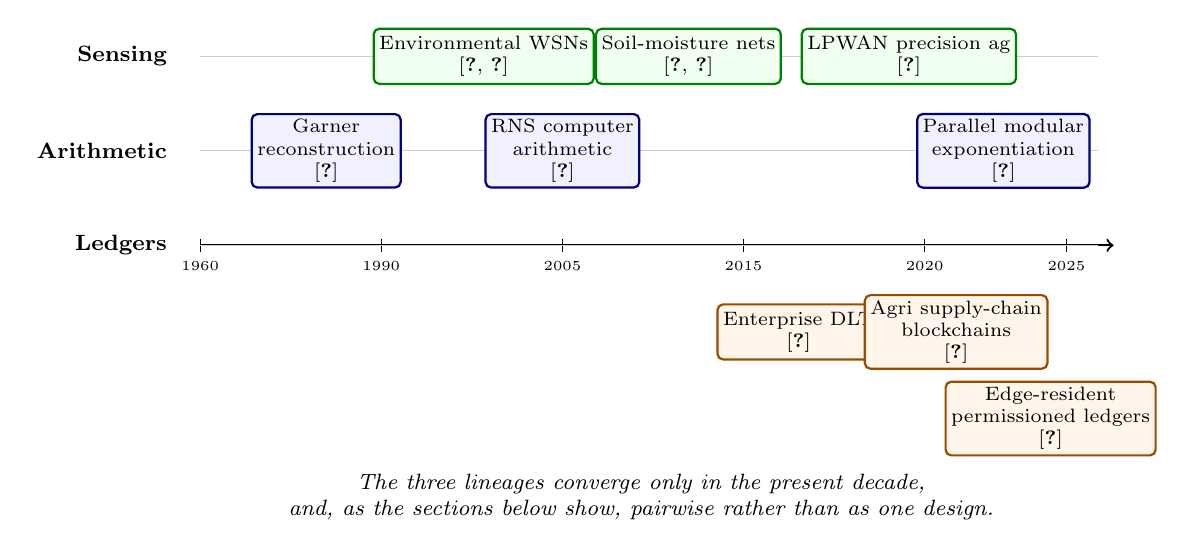
\begin{tikzpicture}[
      lane/.style={font=\footnotesize\bfseries},
      seg/.style={draw, thick, rounded corners=2pt, minimum height=7mm,
                  align=center, font=\scriptsize, inner sep=2pt},
      yr/.style={font=\tiny, align=center}
    ]
    % Axis
    \draw[->, thick] (0,0) -- (11.6,0) node[right, font=\footnotesize]{};
    \foreach \x/\lab in {0/1960, 2.3/1990, 4.6/2005, 6.9/2015, 9.2/2020, 11/2025}
      \draw (\x,0.08) -- (\x,-0.08) node[below, yr]{\lab};

    % Lane 1: agricultural sensing
    \node[lane, anchor=east] at (-0.3,2.4) {Sensing};
    \draw[gray!40, thin] (0,2.4) -- (11.4,2.4);
    \node[seg, fill=green!6, draw=green!50!black] at (3.6,2.4)
      {Environmental WSNs\\\cite{wang2006wireless, pierce1999site}};
    \node[seg, fill=green!6, draw=green!50!black] at (6.2,2.4)
      {Soil-moisture nets\\\cite{bogena2010soil, evans2008precision}};
    \node[seg, fill=green!6, draw=green!50!black] at (9.0,2.4)
      {LPWAN precision ag\\\cite{adelantado2017understanding}};

    % Lane 2: residue arithmetic
    \node[lane, anchor=east] at (-0.3,1.2) {Arithmetic};
    \draw[gray!40, thin] (0,1.2) -- (11.4,1.2);
    \node[seg, fill=blue!6, draw=blue!50!black] at (1.6,1.2)
      {Garner\\reconstruction\\\cite{garner1959residue}};
    \node[seg, fill=blue!6, draw=blue!50!black] at (4.6,1.2)
      {RNS computer\\arithmetic\\\cite{ding1996remainder}};
    \node[seg, fill=blue!6, draw=blue!50!black] at (10.2,1.2)
      {Parallel modular\\exponentiation\\\cite{shoup2009computational}};

    % Lane 3: ledgers
    \node[lane, anchor=east] at (-0.3,0) {Ledgers};
    \draw[gray!40, thin] (0,0) -- (11.4,0.0);
    \node[seg, fill=orange!8, draw=orange!60!black] at (7.6,-1.1)
      {Enterprise DLT\\\cite{christidis2016blockchain}};
    \node[seg, fill=orange!8, draw=orange!60!black] at (9.6,-1.1)
      {Agri supply-chain\\blockchains\\\cite{tian2016agri}};
    \node[seg, fill=orange!8, draw=orange!60!black] at (10.8,-2.2)
      {Edge-resident\\permissioned ledgers\\\cite{tar2023fabric}};

    \node[font=\footnotesize\itshape, align=center] at (5.6,-3.2)
      {The three lineages converge only in the present decade,\\
       and, as the sections below show, pairwise rather than as one design.};
  \end{tikzpicture}
  \caption{Three lineages underlying our work, developed independently
           until converging in the 2020s.}
  \label{fig:lit-timeline}
\end{figure}

\section{Foundations and Enabling Technologies}
\label{sec:lit_foundations}

The four strands below supply the technical vocabulary the rest of the
chapter uses: what a distributed ledger guarantees and at what cost, how
agricultural sensing is instrumented, what the radio charges for a packet,
and what residue arithmetic offers.

\ubsoft{Fundamentals of Blockchain Technology}
\label{subsec:lit_fundamentals}

Before turning to agriculture specifically, we set out what a blockchain
is, because the word covers a wide family of designs and the choice among
them is not cosmetic. A blockchain is, at its simplest, an
append-only ledger replicated across a set of nodes that do not
fully trust one another, ordered into blocks that are cryptographically
chained together~\cite{christidis2016blockchain, debruyne2022trust}. Each
block $B_i$ commits to its predecessor and its own transaction set through
\begin{equation}
h_i = H\!\left( h_{i-1} \,\|\, \mathrm{tx}_i \right),
\label{eq:hash_chain}
\end{equation}
where $H$ is a cryptographic hash function, so that altering any committed
$\mathrm{tx}_j$ for $j \le i$ requires recomputing every $h_j,\ldots,h_i$
across every replica that holds the chain, a cost that grows with the
number of mutually distrusting replicas rather than
shrinking~\cite{fernandez2024iotTamper}. Merkle's original construction
generalises Equation~\ref{eq:hash_chain} to a binary tree of hashes so that
membership of a single transaction can be proven in $O(\log n)$ rather than
by revealing the whole block, a property later systems use for compact
audit proofs~\cite{sharma2018merkle}. This hash-chaining property, not any
particular cryptocurrency, is what the literature means by tamper evidence,
and it is what agricultural applications actually draw on: a record, once
committed and replicated, cannot be silently rewritten by any single party.

Blockchains split first on who may participate. Permissionless (public)
chains such as Bitcoin and Ethereum admit any node and settle disagreement
through open, resource-costly consensus, typically proof of work, so that
attacking the chain costs more than any single participant can
afford~\cite{melo2024unlockingblockchain, anon2024securitysecp}.
Permissioned (private or consortium) chains restrict participation to
identified, vetted members, replacing open competition with a membership
service that binds every submitted transaction to an accountable
identity~\cite{jayaram2023hyperledger, krstic2020hyperledgerframeworks}.
Hyperledger Fabric, the platform we deploy, is representative of
the permissioned family: a \gls{msp} issues \gls{x509} certificates to
every organisation and peer, an execute-order-validate pipeline separates
transaction endorsement from ordering, and chaincode, Fabric's term for a
smart contract, encodes the business logic that peers execute and validate
before a transaction is committed~\cite{jayaram2023hyperledger,
mediumChaincode}. A permissionless design buys resistance to an unknown,
potentially adversarial population of participants at the cost of energy
and finality latency; a permissioned design accepts a smaller, vetted
membership in exchange for finality in seconds rather than minutes and no
mining cost, which is why every agricultural deployment reviewed in this
chapter, without exception, chooses the permissioned family. A consortium
of farms, certifiers and buyers is exactly the setting permissioned
platforms are built for: participants who must cooperate on shared records
without extending one another unconditional trust, and who are identifiable
and accountable rather than anonymous~\cite{debruyne2022trust,
kumar2024collaborativenetworks}.

Smart contracts are the mechanism that turns a passive ledger into an
active one. Once deployed, chaincode executes deterministically on every
endorsing peer, so that business rules, who may submit a reading, what
counts as a valid range, how a certification decision is recorded, are
enforced by consensus over code rather than by a single administrator's
discretion~\cite{krstic2020hyperledgerframeworks, tang2025applicationsblockchain}.
Alternative ledger topologies exist outside the block-and-chain model
proper, directed-acyclic-graph ledgers such as IOTA dispense with blocks
altogether and let each new transaction validate two prior
ones~\cite{anonndimprovedblockchain}, trading the strict global ordering a
blockchain provides for higher throughput under light load; we return to
this trade-off, and to consensus proper, in
Section~\ref{subsec:lit_consensus}. What every variant shares, and what
the rest of this chapter takes as given, is the replicated, hash-chained
record that makes a committed reading expensive to falsify after the fact.
Underlying every transaction's authenticity, in both permissioned and
permissionless designs, is public-key cryptography: a node signs what it
submits with a private key, and peers verify that signature against a
public one before accepting it, typically an elliptic-curve scheme such as
\gls{ecdsa} over the secp256k1 curve~\cite{anon2024securitysecp}. Signature
verification is itself a parallelisable modular-arithmetic computation,
which is the property Section~\ref{subsec:lit_crt} returns to when it
discusses residue number systems.

\ubsoft{Precision Agriculture and Internet of Things Sensing}
\label{subsec:lit_precision_ag}

Precision agriculture research has consistently found that sensing density
and irrigation efficiency move together. \gls{iot} soil and canopy sensing
networks demonstrated early that automated, sensor-driven scheduling
outperforms calendar-based irrigation on both water use and
yield~\cite{rathi2025smart, brooks2019precisionWater, chatterjee2023precision, gondchawar2016agriculture4}, a finding replicated across arid and
semi-arid contexts where the water-saving incentive is
largest~\cite{williams2022savings, miller2020climateImpact, garrido2018mediterranean}. Reviews of the field converge on the same three
limitations. First, decision-support integration remains
fragmented: sensor data reaches a dashboard but rarely a closed-loop
controller with an auditable
rationale~\cite{aydin2021comprehensive, zhang2002precision, gebbers2010precision, mcbratney2005future}. Second, most systems evaluate
the analytics rather than the network that feeds them, so machine-learning
yield and stress models are reported against clean, simulated input streams
rather than the loss and jitter that a field deployment actually
produces~\cite{chlingaryan2018machine, goap2018iot, mohanty2016using, van2020review}. Third, sensing accuracy in the field degrades in ways a
laboratory calibration does not capture, drift, fouling and intermittent
failure among them, and few studies report the resulting error
budget~\cite{akhtar2019sensingAccuracy, agri2024sensorAccuracy, garcia2021sensorFailures, lopez2023remoteFailure}. Later generations of this
literature push toward higher automation, describing four- and
five-generation smart-farming stacks that assume the identity and integrity
of every reading rather than establishing
it~\cite{suleiman2025agriculture5, owusu2025iotAgri, yang2021iotSensing, singh2019iotSmartIrrigation, jin2025productivity}. That assumption is exactly
the gap Section~\ref{subsec:lit_blockchain_ag} returns to.

\ubsoft{Low-Power Wide-Area Network Transmission Optimisation and Energy Modelling}
\label{subsec:lit_lpwan}

\gls{lora} is the dominant physical layer in this literature because it
reaches farm-scale distances, of the order of kilometres in rural terrain,
from a battery node at sub-milliwatt receive
power~\cite{raza2018lorawan, li2020performance, raj2017comprehensive}. The
cost is airtime. The Semtech chirp spread-spectrum design fixes the time to
transmit a payload of $PL$ bytes as a function of spreading factor $\mathrm{SF}$,
bandwidth $\mathrm{BW}$, coding rate $\mathrm{CR}$ and the low-data-rate
optimisation flag $\mathrm{DE}$~\cite{semtech2015lorawan, bor2016lorawan}.
The symbol period is
\begin{equation}
T_{\text{sym}} = \frac{2^{\mathrm{SF}}}{\mathrm{BW}},
\label{eq:lora_symbol}
\end{equation}
the payload requires
\begin{equation}
n_{\text{payload}} = 8 + \max\!\left(
  \left\lceil \frac{8\,PL - 4\,\mathrm{SF} + 28 + 16\,\mathrm{CRC} - 20\,\mathrm{IH}}
                    {4(\mathrm{SF} - 2\,\mathrm{DE})} \right\rceil
  (\mathrm{CR}+4),\; 0 \right)
\label{eq:lora_payload_symbols}
\end{equation}
symbols, and total airtime is
\begin{equation}
T_{\text{air}} = \underbrace{(n_{\text{preamble}} + 4.25)\, T_{\text{sym}}}_{\text{preamble}}
               + n_{\text{payload}} \, T_{\text{sym}}.
\label{eq:lora_airtime}
\end{equation}
Equation~\ref{eq:lora_airtime} is the quantity every optimisation in this
literature ultimately reduces: for a fixed $\mathrm{SF}$ and $\mathrm{BW}$,
airtime is affine in payload length, so a shorter payload is the only lever
available once the modulation is chosen. Regulatory duty-cycle limits then
convert that airtime into a rate ceiling rather than merely an energy cost.
Under \gls{etsi} EN\,300\,220, a sub-GHz node may occupy its channel for at
most a fixed fraction $\mathrm{DC}_{\max}$ of any observation
window~\cite{ttn2024eu868, loraalliance2021regional}, so a single reading
consumes
\begin{equation}
\mathrm{DC} = \frac{T_{\text{air}}}{T_{\text{window}}} \leq \mathrm{DC}_{\max},
\label{eq:duty_cycle}
\end{equation}
and offered channel load across $N$ nodes reporting once per window is
$G = N\,T_{\text{air}}/T_{\text{window}}$ Erlang, which under the pure-ALOHA
assumption common to this literature bounds per-packet collision probability
at $P_{\text{coll}} = 1 - e^{-2G} \approx 2G$ for small
$G$~\cite{bor2016lorawan, adelantado2017understanding}. Node energy per
transmission follows directly, $E_{\text{tx}} = P_{\text{tx}}\,T_{\text{air}}$,
so any reduction in $T_{\text{air}}$ is simultaneously an energy saving and a
capacity gain, which is why the transmission-optimisation literature and the
energy-modelling literature are, in practice, one
body of work~\cite{barr1994energy, polastre2005versatile, gonzalez2000energy, mohammed2025loraEnergy, sanchez2021energy, heinzelman2000energy}.

Two families of technique attack Equation~\ref{eq:lora_airtime} from
opposite sides, summarised in Figure~\ref{fig:lit-transmission-taxonomy}.
\textbf{Compression} keeps one packet per reading and shrinks $PL$: general
lossless coders such as Huffman and Lempel-Ziv-Welch adapted to sensor
streams~\cite{li2018lossless, marcelloni2009energy, ziv1977universal, huffman1952method, salomon2007data} report 20 to 40\% payload reduction but
require dictionary or frequency-table state that a microcontroller with a
few kilobytes of free \gls{ram} can only marginally
afford~\cite{chen2025compression, lzw_dictionary_size}, and adaptive
sampling reduces transmitted volume by skipping readings, which risks
missing the threshold event the network exists to
detect~\cite{kjellsson2008adaptive}. \textbf{Decomposition} takes the
opposite path: it accepts more packets in exchange for each one being
far shorter, splitting a reading across parallel channels rather than
compressing it on one. Residue-based decomposition for wireless sensor
data has been explored for storage reduction and for wireless sensor
network lifetime~\cite{vidhya2021crt, khan2023fuzzycrt, rahman2022rnsenergy, djeddi2025parallelCRT}, but, as
Section~\ref{subsec:lit_crt} details, not for exploiting a multi-channel
concentrator's ability to demodulate several sub-channels
\emph{simultaneously}, which is the specific mechanism we study.
LoRa-specific network-capacity work independently confirms that channel
occupancy, not raw byte count, is the binding constraint on
gateway-served node population~\cite{centenaro2016lorawanlimits, zhang2022lorawan, chapungo2025lorawan, bicamumakuba2025lorawan, turlykozhayeva2024proactive, mozambique2021lorawan}, which is the same
quantity Equation~\ref{eq:duty_cycle} fixes.

\begin{figure}[htbp]
  \centering
  \begin{tikzpicture}[
      root/.style={draw, thick, rounded corners=2pt, fill=black!5,
                   font=\small\bfseries, align=center, minimum width=42mm,
                   minimum height=8mm},
      branch/.style={draw, rounded corners=2pt, font=\footnotesize\bfseries,
                     align=center, minimum width=38mm, minimum height=8mm},
      leaf/.style={draw, rounded corners=2pt, font=\scriptsize, align=center,
                   text width=30mm, minimum height=11mm, inner sep=2pt},
      e/.style={-{Stealth[length=1.8mm]}, thick, draw=black!60}
    ]
    \node[root] (r) at (0,4.4) {Reduce airtime\\$T_{\text{air}}$ (Eq.~\ref{eq:lora_airtime})};

    \node[branch, fill=red!6, draw=red!55!black] (c) at (-4.2,2.6) {Compression\\(one packet)};
    \node[branch, fill=blue!6, draw=blue!55!black] (d) at (4.2,2.6) {Decomposition\\(many packets)};
    \draw[e] (r.south) -- ++(0,-0.4) -| (c.north);
    \draw[e] (r.south) -- ++(0,-0.4) -| (d.north);

    \node[leaf, fill=red!4] (c1) at (-6.0,0.6) {Dictionary coders\\(LZW, Huffman)\\\cite{li2018lossless, marcelloni2009energy}};
    \node[leaf, fill=red!4] (c2) at (-2.4,0.6) {Adaptive\\sampling\\\cite{kjellsson2008adaptive}};
    \draw[e] (c.south) -- ++(0,-0.4) -| (c1.north);
    \draw[e] (c.south) -- ++(0,-0.4) -| (c2.north);

    \node[leaf, fill=blue!4] (d1) at (2.4,0.6) {Residue storage\\\ \& lifetime\\\cite{vidhya2021crt, rahman2022rnsenergy}};
    \node[leaf, fill=blue!4] (d2) at (6.0,0.6) {Multi-channel\\parallel reception\\(our work)};
    \draw[e] (d.south) -- ++(0,-0.4) -| (d1.north);
    \draw[e] (d.south) -- ++(0,-0.4) -| (d2.north);

    \node[font=\footnotesize\itshape, text width=105mm, align=center] at (0,-1.7)
      {Compression shrinks the payload on one channel; decomposition trades
       packet count for per-packet occupancy across several. The literature
       has developed the left branch thoroughly and the right branch for
       storage and lifetime, but not yet for concurrent multi-channel
       reception.};
  \end{tikzpicture}
  \caption{Transmission-efficiency strategies for constrained \gls{iot}
           radios; we occupy the open leaf on the right.}
  \label{fig:lit-transmission-taxonomy}
\end{figure}

Table~\ref{tab:lit-lpwan-comparison} summarises representative results
across both branches on the metric that matters for gateway capacity,
per-packet airtime or its energy equivalent, rather than the compression
ratio each source reports on its own terms.

\begin{table}[htbp]
\centering
\caption{Representative low-power wide-area transmission-efficiency results}
\label{tab:lit-lpwan-comparison}
\footnotesize
\begin{tabularx}{\textwidth}{@{}p{0.21\textwidth}p{0.18\textwidth}X@{}}
\toprule
\textbf{Study} & \textbf{Technique} & \textbf{Reported limitation} \\
\midrule
Li and Simonot-Lion~\cite{li2018lossless};\\ Marcelloni and Vecchio~\cite{marcelloni2009energy}
  & Huffman/LZW sensor compression
  & Dictionary or frequency-table state exceeds the free \gls{ram} of the
    smallest microcontroller class; ratio degrades on low-entropy sensor
    streams \\
\midrule
Kjellsson et al.~\cite{kjellsson2008adaptive}
  & Adaptive, event-driven sampling
  & Reduces volume, not per-packet occupancy; risks missing threshold
    events between samples \\
\midrule
Vidhya and Brindha~\cite{vidhya2021crt}
  & \gls{crt} residue image compression
  & Targets storage footprint, not transmission concurrency; single-channel
    model \\
\midrule
Buttigieg et al.~\cite{khan2023fuzzycrt};\\ Pourbigharaz and Yassine~\cite{rahman2022rnsenergy}
  & \gls{rns} energy reduction in \glspl{wsn}
  & Energy accounting only; no gateway-capacity or multi-channel reception
    model \\
\midrule
Ye et al.~\cite{djeddi2025parallelCRT}
  & \gls{rns}-based reliable \gls{wsn} transmission
  & Reliability under loss, not concurrent channel exploitation \\
\bottomrule
\end{tabularx}
\end{table}

\ubsoft{Residue Number Systems and the Chinese Remainder Theorem in Communications}
\label{subsec:lit_crt}

The theorem itself is unconditional. For pairwise coprime moduli
$m_1,\ldots,m_k$ and $M = \prod_{i=1}^{k} m_i$, every integer
$x \in [0,M)$ is uniquely determined by its residue vector
$(r_1,\ldots,r_k)$, $r_i = x \bmod m_i$~\cite{garner1959residue, hardy2008introduction}. Garner's algorithm reconstructs $x$ from the
residues in closed form,
\begin{equation}
x = \left( \sum_{i=1}^{k} r_i\, M_i\, N_i \right) \bmod M, \qquad
M_i = \frac{M}{m_i}, \quad N_i = M_i^{-1} \bmod m_i,
\label{eq:crt_reconstruction}
\end{equation}
exact because $M_i N_i \equiv 1 \pmod{m_i}$ by
construction~\cite{garner1959residue, knuth1997art}, and computable in
$O(k)$ modular multiplications regardless of the magnitude of $x$, which is
the property that later work in residue number systems generalised into a
programme for fast, carry-free, parallel
arithmetic~\cite{ding1996remainder, parhami2010computer}. A second
property of Equation~\ref{eq:crt_reconstruction} bears on reliability
rather than speed. Goldreich, Ron and Sudan formalised the error-tolerant
case, showing that $x$ remains recoverable from a strict subset of
residues under bounded corruption, "Chinese remaindering with
errors"~\cite{goldreich1999china}, a result later systematised alongside
subset-product reconstruction in computational number
theory~\cite{shoup2009computational}. That subset-recovery property is a
statement about \emph{reconstruction}, not about \emph{disclosure}: it is
tempting to read a residue set as a threshold secret-sharing scheme, exact
recovery from a complete or near-complete subset, negligible information
from any one share in isolation, but the two constructions are not
equivalent. A Shamir-style share is deliberately randomised so that any
share short of the threshold is uniformly distributed independent of the
secret~\cite{shoup2009computational}; a plain \gls{crt} residue is not.
$r_i = x \bmod m_i$ is a deterministic function of $x$, so intercepting it
narrows the field of possible values by a factor of roughly $m_i$ rather
than leaking nothing, and if the plaintext domain is itself small relative
to $m_i$, a single residue can narrow that field to very little uncertainty
indeed. Whether residue disclosure is negligible in practice therefore
depends on the ratio between the plaintext's domain and the moduli chosen,
not on the reconstruction identity alone, and no prior work has
established that ratio for any deployed system;
Section~\ref{subsec:lit_privacy} returns to this distinction, and Chapter
One's hypothesis H5 treats it as open rather than established.

Two application communities have used Equation~\ref{eq:crt_reconstruction}
for two different resources, and both stop short of a shared wireless
channel. The first treats it as a \emph{storage} problem: residue-based
lossless image compression reports 15 to 30\% footprint reduction with
exact reconstruction~\cite{vidhya2021crt}. The second treats it as an
\emph{energy} problem inside wireless sensor networks, converting a
single wide-range reading into several narrow-range residues to shrink the
arithmetic and storage cost per node~\cite{rahman2022rnsenergy,
khan2023fuzzycrt, djeddi2025parallelCRT}. Neither treats the residues as
packets to be received concurrently on separate radio channels; both keep
the decomposition on one device (compressing what is stored) or across one
uplink (reducing what one node computes and sends), rather than exploiting
a multi-channel concentrator's ability to demodulate several sub-channels
\emph{simultaneously}. To our knowledge, no published system applies
residue decomposition to concurrent multi-channel radio reception, which
is the gap Chapter Three's design addresses. Figure~\ref{fig:lit-crt-applications}
lays the three resources side by side: two are established in the
literature just surveyed, the third is open.

\begin{figure}[htbp]
  \centering
  \begin{tikzpicture}[
      root/.style={draw, thick, rounded corners=2pt, fill=black!5,
                   font=\small\bfseries, align=center, minimum width=64mm,
                   minimum height=8mm},
      branch/.style={draw, rounded corners=2pt, font=\scriptsize, align=center,
                     text width=36mm, minimum height=17mm, inner sep=2pt},
      e/.style={-{Stealth[length=1.8mm]}, thick, draw=black!60}
    ]
    \node[root] (r) at (0,3.2) {Residue decomposition\\(Eq.~\ref{eq:crt_reconstruction})};

    \node[branch, fill=blue!5, draw=blue!50!black] (storage) at (-6.4,0.8)
      {\textbf{Storage}\\one device, one image\\15-30\% footprint
       reduction~\cite{vidhya2021crt}};
    \node[branch, fill=blue!5, draw=blue!50!black] (energy) at (-1.6,0.8)
      {\textbf{Energy}\\one uplink, one node\\per-node arithmetic and
       storage cost~\cite{rahman2022rnsenergy, khan2023fuzzycrt}};
    \node[branch, dashed, fill=red!4, draw=red!55!black] (comms) at (4.8,0.8)
      {\textbf{Radio concurrency}\\several channels, one\\concentrator,
       received \emph{simultaneously}\\\emph{not established, addressed
       in Chapter Three}};

    \draw[e] (r.south) -- ++(0,-0.4) -| (storage.north);
    \draw[e] (r.south) -- ++(0,-0.4) -| (energy.north);
    \draw[e] (r.south) -- ++(0,-0.4) -| (comms.north);

    \node[font=\footnotesize\itshape, text width=118mm, align=center] at (-0.8,-2.1)
      {Both established applications keep the decomposition on one device
       or one uplink; neither exploits concurrent reception across a
       multi-channel concentrator, which is the resource this thesis
       spends the decomposition on.};
  \end{tikzpicture}
  \caption{The three resources residue decomposition has been applied to;
           radio concurrency remains open in the surveyed literature.}
  \label{fig:lit-crt-applications}
\end{figure}

Residue number systems have a third, older home outside networking
entirely: fast computer arithmetic and hardware design, where the absence
of carry propagation across residue channels makes addition and
multiplication in each channel independent of every other, at the cost of
comparison and division becoming hard~\cite{ding1996remainder,
parhami2010computer}. That same independence gives residue codes a natural
fault-tolerance reading, since a corrupted or missing channel affects only
the value it encodes rather than propagating a carry error into its
neighbours, which is part of why redundant residue codes have long been
used for error detection in
hardware~\cite{knuth1997art, hardy2008introduction}. The parallelism this
independence buys is architecturally the same kind of parallelism that the
blockchain-scalability literature pursues by partitioning transaction load
across shards or channels rather than processing it as one serial
stream~\cite{horvath2025assistedsharding, anonndoptimizedcloud}: both
decompose a workload into independently processable parts and pay a
bounded recombination cost to reassemble the result. We are not aware of
published work that states this parallel explicitly or that applies
residue decomposition to a blockchain-connected radio link;
Section~\ref{subsec:lit_scalability} returns to the blockchain side of
that comparison once the scalability literature itself has been surveyed.

\section{Literature Specific to the Topic}
\label{sec:lit_specific_topic}

Where the foundations are general, the work below sits directly on the
problem this thesis addresses, and is grouped by the property it tries to
secure.

\ubsoft{Blockchain and Distributed Ledger Technology in Agriculture and Supply Chains}
\label{subsec:lit_blockchain_ag}

Section~\ref{subsec:lit_fundamentals} sets out the hash-chaining identity
(Equation~\ref{eq:hash_chain}) that gives a replicated ledger its tamper
evidence. Applied to agriculture, this tamper-evidence property has been
used for supply-chain
transparency~\cite{tian2016agri, kamilaris2019rise, oh2025foodsafety, galvez2018future, tian2017traceability, reyna2018blockchain, tian2017agri, anonndsupplychain}, farm-data
management~\cite{lin2018blockchain, ferrag2020security, haque2024scalable, zhang2019blockchain, ali2023farmDataTampering}, and smart-contract
automation of certification and payment
logic~\cite{rama2021systematic, patil2022blockchain, nguyen2022smartFarmingSC, tian2017agri}. Cross-organisational data
sharing has more recently been framed through self-sovereign identity,
letting a farm operator authorise fine-grained access without handing a
consortium a standing credential~\cite{amraouy2025ssi}, and water-quality
and irrigation-specific ledgers report similar tamper-evidence
gains~\cite{saito2025blockchainWaterQuality, arshad2022blockchainBenefits, ali2023farmDataTampering, rahman2019agriSecurity}. The generic \gls{iot}-blockchain integration
literature that agricultural systems draw their architecture from
independently confirms the same design pattern: a lightweight device signs
and forwards, a gateway or edge node validates and submits, and the ledger
anchors a hash rather than the raw
payload~\cite{dorri2017blockchain, nguyen2019blockchain, xu2020making, reyna2018blockchain, benedict2021decentralized}.

Crop- and commodity-specific traceability deployments give this pattern
concrete form. \textcite{salah2019blockchain} traces soybean shipments end
to end on Ethereum, anchoring custody transfers as they cross the supply
chain; a comparable case study for ginger in Nepal reports the same
design applied to a smallholder export
crop~\cite{anonndblockchainbased}, and a pilot study of blockchain for
agriculture and food more broadly finds the technology's actual value
concentrated in dispute resolution and recall speed rather than in the
blockchain mechanism's novelty as such~\cite{liu2021traceableSupply}.
Reviews that step back from individual case studies converge on
transparency and traceability as the two benefits every deployment claims,
whatever the crop~\cite{anonndblockchaintechnology2}, and on collaborative
trust and cross-party transparency as the property that justifies choosing
a shared ledger over a conventional shared database in the first
place~\cite{kumar2024collaborativenetworks}. A feasibility analysis of
blockchain and \gls{iot} for African agricultural food supply
chains~\cite{tang2024feasibility} is the closest match in this corpus to
our own deployment context: it names intermittent connectivity, low
digital literacy and capital cost, rather than the blockchain mechanism
itself, as the binding constraints on adoption, which is consistent with
the constrained-hardware and field-deployment focus of Chapter Three's
methodology and reinforces why we evaluate on the low-cost, battery and
solar-powered hardware class that a smallholder deployment can actually
afford, rather than on server-class infrastructure.

What this body of literature does not establish is where the tamper
evidence begins. Almost every system surveyed authenticates at the gateway
or the enterprise boundary and treats the sensor as an untrusted data
source whose values are accepted once they arrive, not a principal whose
identity is bound to the record it produced~\cite{lin2020blockchain, ferrag2020blockchain, kamilaris2019rise, ali2023farmDataTampering}. Table~\ref{tab:lit-blockchain-ag} makes this
concrete across a representative sample: the column that is consistently
weak or absent is node-level, rather than gateway-level, identity binding,
which is precisely the gap Chapter One's problem statement
(Section~\ref{sec:problem}) identifies.

\begin{table}[htbp]
\centering
\caption{Representative blockchain-in-agriculture systems by authentication
         boundary and evaluation setting}
\label{tab:lit-blockchain-ag}
\footnotesize
\begin{tabularx}{\textwidth}{@{}p{0.24\textwidth}p{0.19\textwidth}p{0.16\textwidth}X@{}}
\toprule
\textbf{Study} & \textbf{Authentication boundary} & \textbf{Evaluation setting} & \textbf{Reported gap} \\
\midrule
Tian~\cite{tian2016agri}; Kamilaris et al.~\cite{kamilaris2019rise}
  & Enterprise / consortium & Conceptual, no field data
  & No per-sensor identity; throughput not characterised on constrained hardware \\
\midrule
Zhang et al.~\cite{zhang2019blockchain}
  & Gateway & Simulation
  & Consensus cost assumed server-class hardware \\
\midrule
Amraouy et al.~\cite{amraouy2025ssi}
  & Farm operator (self-sovereign identity)
  & Prototype
  & Access-sharing framework; no edge-hardware performance data \\
\midrule
Reyna et al.~\cite{reyna2018blockchain}; Dorri et al.~\cite{dorri2017blockchain}
  & Generic \gls{iot} gateway & Survey / architecture
  & Identifies the sensor-to-gateway trust gap without closing it \\
\bottomrule
\end{tabularx}
\end{table}

\ubsoft{Edge-Resident Consensus and Constrained-Hardware Ledgers}
\label{subsec:lit_consensus}

Running a permissioned ledger on gateway-class hardware raises a question
the enterprise blockchain literature rarely poses: whether consensus can
complete inside the timing budget of a real-time control loop, on a device
with an order of magnitude less memory and \gls{cpu} throughput than the
server hardware that literature assumes~\cite{tar2023fabric, jayaram2023hyperledger, ibmFabric}. Hyperledger Fabric's execute-order-validate
architecture separates transaction endorsement from ordering, letting an
ordering service reach agreement on transaction sequence rather than
transaction content, and the Raft ordering service we use
implements crash-fault-tolerant, not Byzantine-fault-tolerant,
agreement~\cite{ongaro2014raft, orderingServiceDoc}. The distinction has a
direct complexity consequence. \gls{cft} protocols such as Raft reach
agreement with $O(n)$ message exchanges per decision and tolerate
$f = \lfloor (n-1)/2 \rfloor$ stopped nodes, whereas classical
\gls{bft} protocols such as \gls{pbft} require $n \geq 3f+1$ replicas,
so they tolerate the smaller
$f = \lfloor (n-1)/3 \rfloor$, at $O(n^2)$ messages per decision, to
withstand arbitrary, not merely crash, node
behaviour~\cite{castro1999practical, ongaro2014raft}. A five-node
cluster therefore tolerates two stopped nodes under Raft but only one
Byzantine node under \gls{pbft}, a smaller fault budget bought at a
quadratically larger message cost. Linear-complexity \gls{bft} variants
such as HotStuff
close much of that gap for adversarial settings~\cite{yin2019hotstuff}, and
the state-machine-replication literature more broadly treats the
\gls{cft}/\gls{bft} choice as a trade between message cost and the
threat model tolerated~\cite{bessani2014state}. Deployed on a
consortium of trusted, physically secured gateways rather than an open or
adversarial network, we adopt \gls{cft} for that reason, a choice the
consensus literature supports for permissioned agricultural
settings~\cite{dube2024fabricIrrigation} but rarely evaluates on
gateway-class \gls{arm64} hardware in the field, as
Table~\ref{tab:lit-consensus} shows.

\begin{figure}[htbp]
  \centering
  \begin{tikzpicture}[
      root/.style={draw, thick, rounded corners=2pt, fill=black!5, font=\small\bfseries,
                   align=center, minimum width=46mm, minimum height=8mm},
      branch/.style={draw, rounded corners=2pt, font=\footnotesize\bfseries,
                     align=center, minimum width=40mm, minimum height=8mm},
      leaf/.style={draw, rounded corners=2pt, font=\scriptsize, align=center,
                   text width=34mm, minimum height=13mm, inner sep=2pt},
      e/.style={-{Stealth[length=1.8mm]}, thick, draw=black!60}
    ]
    \node[root] (r) at (0,4.2) {Fault model tolerated};

    \node[branch, fill=teal!6, draw=teal!55!black] (cft) at (-4.6,2.4) {Crash-fault\\tolerant};
    \node[branch, fill=purple!6, draw=purple!55!black] (bft) at (4.6,2.4) {Byzantine-fault\\tolerant};
    \draw[e] (r.south) -- ++(0,-0.4) -| (cft.north);
    \draw[e] (r.south) -- ++(0,-0.4) -| (bft.north);

    \node[leaf, fill=teal!4] (l1) at (-4.6,0.2)
      {Raft\\$O(n)$ msgs/decision\\$f=\lfloor(n-1)/2\rfloor$\\\cite{ongaro2014raft}\\\emph{used in our design}};

    \node[leaf, fill=purple!4] (l2) at (2.2,0.2)
      {\gls{pbft}\\$O(n^2)$ msgs/decision\\$f=\lfloor(n-1)/3\rfloor$\\\cite{castro1999practical}};
    \node[leaf, fill=purple!4] (l3) at (7.0,0.2)
      {HotStuff\\$O(n)$ msgs/decision,\\linear view-change\\\cite{yin2019hotstuff}};
    \draw[e] (bft.south) -- ++(0,-0.4) -| (l2.north);
    \draw[e] (bft.south) -- ++(0,-0.4) -| (l3.north);

    \node[font=\footnotesize\itshape, text width=110mm, align=center] at (0,-2.0)
      {Message complexity scales with the fault model tolerated, not with
       hardware class. \gls{cft} is adopted here because the deployment is a
       trusted, physically secured consortium; prior work rarely reports
       which choice was measured on \gls{arm64} gateway
       hardware rather than assumed server-class hardware.};
  \end{tikzpicture}
  \caption{Consensus fault models and their message complexity, after
           \cite{ongaro2014raft, castro1999practical, yin2019hotstuff, bessani2014state}.}
  \label{fig:lit-consensus-taxonomy}
\end{figure}

Whichever protocol is chosen, its saturation behaviour under load is
standard queueing theory. Treating packet or transaction arrivals as
Poisson and service time as deterministic (an M/D/1 queue), mean waiting
time before service is
\begin{equation}
W_q = \frac{\rho}{2(1-\rho)}\, T_{\text{service}}, \qquad
\rho = \lambda\, T_{\text{service}},
\label{eq:mdOne}
\end{equation}
where $\lambda$ is the arrival rate and $T_{\text{service}}$ the
deterministic service time, so that total latency $L = T_{\text{service}} +
W_q$ is flat while $\rho \ll 1$ and diverges as $\rho \to 1$. The
scalability literature for both LoRa gateways and blockchain orderers uses
Equation~\ref{eq:mdOne}, or its close relatives, to project a saturation
point from a small deployment rather than requiring one at
scale~\cite{jayaram2023hyperledger, pinto2024throughput, cui2023ipfsFabric, rahimi2023fabricSensors, khan2021fabricCRT}, but, as with the consensus
literature above, validation against real field load rather than synthetic
benchmark load remains the exception rather than the
rule. The \gls{cap} theorem underlies the same trade from a different
angle: no distributed data store can simultaneously guarantee consistency
and availability under network partition~\cite{brewer2000towards, gilbert2002brewer}, and permissioned ledgers on intermittently connected
rural gateways sit squarely inside that trade-off, a point the
practitioner literature on eventual, \gls{acid}-relaxed consistency in
distributed systems makes explicit~\cite{pritchett2008base}.

\begin{table}[htbp]
\centering
\caption{Consensus and edge-ledger literature by hardware class evaluated}
\label{tab:lit-consensus}
\footnotesize
\begin{tabularx}{\textwidth}{@{}p{0.22\textwidth}p{0.18\textwidth}p{0.14\textwidth}X@{}}
\toprule
\textbf{Study} & \textbf{Protocol} & \textbf{Hardware class} & \textbf{Reported gap} \\
\midrule
Ongaro and Ousterhout~\cite{ongaro2014raft}
  & Raft (\gls{cft})
  & Server-class (original)
  & Correctness and understandability proof; no constrained-hardware
    evaluation \\
\midrule
Castro and Liskov~\cite{castro1999practical}
  & \gls{pbft} (\gls{bft})
  & Server-class
  & $O(n^2)$ messaging cost not evaluated against gateway bandwidth \\
\midrule
Androulaki et al.~\cite{jayaram2023hyperledger}
  & Fabric E-O-V pipeline
  & Data-centre reference deployment
  & Throughput figures not reproduced on \gls{arm64} \\
\midrule
Rahimi et al.~\cite{rahimi2023fabricSensors}; Cui et al.~\cite{cui2023ipfsFabric}
  & Fabric + sensor / off-chain storage
  & Prototype, short-duration
  & No sustained field deployment; saturation point not field-validated \\
\bottomrule
\end{tabularx}
\end{table}

\ubsoft{Identity, Access Control and Privacy-Preserving Data Processing}
\label{subsec:lit_privacy}

Two threads meet here: how a permissioned ledger decides who may act, and
how it protects what a record discloses to parties who are entitled to see
that it exists but not what it contains. On the first thread, \gls{rbac}
enforced in chaincode is the standard mechanism, with permissions attached
to roles rather than individual identities and a \gls{msp} resolving each
transaction's submitter to a role through its
\gls{x509} certificate~\cite{mdpiAccessControl, hyperledger2022msp}. Flat
\gls{rbac} is the common case in this literature: a fixed set of roles,
each with a fixed permission set, checked at the point a transaction is
submitted. Administrative role hierarchies, in which a senior role
inherits every permission of the roles beneath it in a partial order, are
well established in access-control theory more broadly and are used to
express exactly this kind of inheritance without duplicating permission
assignments across roles~\cite{lu2022revocation}. What the Fabric
access-control literature consistently shows, hierarchical or not, is that
enforcement happens at the \emph{gateway}, the device holding the
\gls{x509} certificate that signs the transaction, not at the individual
sensing node whose reading the transaction
carries~\cite{mdpiAccessControl, yavari2020blockchain}. An improved
blockchain-based authentication protocol for \gls{iot} network management
pushes credential issuance closer to the device but still assumes a
network manager mediates enrolment rather than the constrained node
enrolling itself~\cite{yavari2020blockchain}. Certificate revocation
latency under this model has been measured directly, with propagation
delay across a small gossip-connected peer set on the order of minutes
rather than seconds~\cite{lu2022revocation}, a figure we reproduce
independently in Chapter Four rather than merely assume. We develop a
hierarchical role structure that closes the node-level identity gap this
literature leaves open, formalised in Appendix~\ref{app:hrbac_matrix} and
implemented in Chapter Three, rather than presented here as part of the
literature under review. Figure~\ref{fig:lit-identity-flow} places that
gap on the enforcement pipeline this literature otherwise establishes.

\begin{figure}[htbp]
  \centering
  \begin{tikzpicture}[
      box/.style={draw, rounded corners=2pt, align=center, font=\scriptsize,
                  minimum height=11mm, text width=21mm, inner sep=3pt},
      stg/.style={box, fill=black!4},
      flow/.style={-{Stealth[length=2mm]}, thick},
      note/.style={font=\footnotesize\itshape, align=center, text width=118mm}
    ]
    \node[stg] (node)   at (0,0)     {Sensing node\\produces a reading};
    \node[stg] (gw)     at (3.0,0)   {Gateway holds\\\gls{x509} certificate};
    \node[stg] (msp)    at (6.0,0)   {\gls{msp} resolves\\certificate to role};
    \node[stg] (rbac)   at (9.0,0)   {\gls{rbac} check\\in chaincode};
    \node[stg] (ledger) at (12.0,0)  {Transaction\\committed};

    \draw[flow, dashed, red!55!black] (node) -- (gw);
    \draw[flow] (gw) -- (msp);
    \draw[flow] (msp) -- (rbac);
    \draw[flow] (rbac) -- (ledger);

    \begin{scope}[on background layer]
      \node[draw, dashed, thick, red!55!black, rounded corners=3pt,
            fit=(node), inner sep=2.5mm] {};
    \end{scope}
    \node[font=\footnotesize\itshape, align=center] (gaplabel) at (0,-1.6)
      {identity gap};

    \node[note] at (6.0,-2.6)
      {Enforcement in this literature begins at the gateway's certificate,
       hierarchical or not; the sensing node that produced the reading
       carries no credential of its own.};
  \end{tikzpicture}
  \caption{Where identity enforcement begins in the surveyed access-control
           literature, and the node-level gap it leaves.}
  \label{fig:lit-identity-flow}
\end{figure}

On the second thread, privacy in a replicated ledger is structurally
difficult: the same replication that gives every consortium member a
tamper-evident copy of a record also gives every member a copy of whatever
that record discloses. Off-chain storage with an on-chain hash anchor is
the common mitigation, verifiable without being
world-readable~\cite{kim2023privacy}, and self-sovereign identity schemes
extend the same principle to access itself, letting a data owner grant and
revoke visibility without a standing
credential~\cite{amraouy2025ssi}. Neither line of work, however, asks
whether the transmission layer itself can contribute to confidentiality
before a record ever reaches the ledger. Section~\ref{subsec:lit_crt}
showed why that question is harder than it first looks: reconstruction
tolerates a missing residue under Goldreich, Ron and Sudan's
error-tolerant formulation~\cite{goldreich1999china}, but a plain
\gls{crt} residue is not a randomised secret share, so subset-recovery
tolerance does not, by itself, establish subset-disclosure
resistance~\cite{shoup2009computational}. What it establishes instead is
a precise condition worth testing rather than assuming: disclosure from
an intercepted residue is bounded by how far the plaintext's domain
exceeds the missing moduli's product, so confidentiality is a property of
the deployed moduli-to-domain ratio, not of the reconstruction identity
in the abstract. Prior work has developed residue decomposition and
threshold secret sharing in separate communities
without stating that condition, which is exactly why Chapter One frames
it as hypothesis H5 rather than a settled result: the rationale
(Section~\ref{sec:rationale}) proposes residue decomposition as a
candidate confidentiality substrate, and H5 requires either a quantified
leakage bound for the deployed moduli and sensor ranges, or an added
randomisation step, before the substrate can be called established.

\ubsoft{Blockchain Scalability and the Parallelism Argument}
\label{subsec:lit_scalability}

A substantial body of recent work attacks ledger throughput directly, and it
matters here because the parallelisation argument we make for the radio link
in Chapter Three has an established precedent in this literature: partition a
workload, process the parts independently, and pay a bounded cost to
recombine them.

\paragraph{Partitioning and sharding.}

Sharding partitions state and transaction load across sub-committees so that
disjoint transactions commit concurrently. Recent treatments add adaptive
assignment of accounts to shards~\cite{horvath2025assistedsharding} and survey
the cost, chiefly cross-shard coordination, which grows with the fraction of
transactions touching more than one partition~\cite{anonndscalabilitysolutions}.
\textcite{maiwada2024techniquesimprove} and
\textcite{maiwada2025blockchainscalability} analyse Bitcoin throughput under
transaction-adjournment and related scheduling techniques, reporting the
familiar result that raw block-level parallelism is bounded by the
serialisation the consensus protocol imposes; an unrelated study of Bitcoin's
own \gls{utxo} transaction patterns reaches the same conclusion from the
storage side, showing that throughput and storage growth trade against one
another however the workload is scheduled~\cite{melo2024unlockingblockchain}.
Layer-two constructions move the work off chain entirely and settle in
aggregate~\cite{patel2023blockchainlayer}, hierarchical models have been
used to characterise where the resulting systems
saturate~\cite{sadath2024scalabilityperformance}, and cloud-hosted
blockchain frameworks pursue the same throughput goal by scaling the
underlying infrastructure rather than the protocol, trading a capital cost
for a scalability
one~\cite{anonndoptimizedcloud}. Multi-chain architectures, keeping
several independent ledgers for different record types and coordinating
across them only where required, are a further partitioning strategy
outside the classic sharding literature, illustrated by a judicial
case-management system that keeps case records and evidentiary records on
separate chains~\cite{alyas2025multiblockchain}.

\paragraph{The common structure of these results.}

Every one of these mechanisms decomposes a workload into parts that can be
processed independently and recombines the parts afterwards, and in every case
the recombination cost is what bounds the gain. That is structurally the same
shape as a residue decomposition, where the recombination is
Equation~\ref{eq:crt_reconstruction} and its cost is $O(k)$, known in advance
and independent of the data, as Section~\ref{subsec:lit_crt} observes. None of
the scalability studies surveyed here states that parallel explicitly, and
none applies a residue decomposition to the workload it partitions; the
common structure is, to our knowledge, an observation this review is making
by reading the two literatures side by side, not a result either literature
has published. Whether the same recombination-bounded-gain argument holds one
layer down, applied to a radio link's channel occupancy rather than a
ledger's transaction load, is a question Chapter Three's design takes up.
Figure~\ref{fig:lit-partition-recombine} sets the four instances against the
one shared pattern.

\begin{figure}[htbp]
  \centering
  \begin{tikzpicture}[
      root/.style={draw, thick, rounded corners=2pt, fill=black!5,
                   font=\small\bfseries, align=center, minimum width=100mm,
                   minimum height=8mm},
      branch/.style={draw, rounded corners=2pt, font=\scriptsize, align=center,
                     text width=26mm, minimum height=17mm, inner sep=2pt},
      e/.style={-{Stealth[length=1.8mm]}, thick, draw=black!60}
    ]
    \node[root] (r) at (0,3.2)
      {Partition workload, process parts independently,\\recombine at
       bounded cost};

    \node[branch, fill=orange!6, draw=orange!60!black] (shard) at (-5.6,0.8)
      {\textbf{Sharding}\\state/transactions across
       sub-committees~\cite{horvath2025assistedsharding}};
    \node[branch, fill=orange!6, draw=orange!60!black] (l2) at (-1.9,0.8)
      {\textbf{Layer-two /\\multi-chain}\\settle off-chain, or split
       record types~\cite{patel2023blockchainlayer, alyas2025multiblockchain}};
    \node[branch, fill=orange!6, draw=orange!60!black] (cloud) at (1.9,0.8)
      {\textbf{Cloud-hosted\\scaling}\\infrastructure scaled, not the
       protocol~\cite{anonndoptimizedcloud}};
    \node[branch, dashed, fill=red!4, draw=red!55!black] (crt) at (5.6,0.8)
      {\textbf{Residue\\decomposition}\\radio-link channel occupancy;
       \emph{not applied here, addressed in Chapter Three}};

    \draw[e] (r.south) -- ++(0,-0.4) -| (shard.north);
    \draw[e] (r.south) -- ++(0,-0.4) -| (l2.north);
    \draw[e] (r.south) -- ++(0,-0.4) -| (cloud.north);
    \draw[e] (r.south) -- ++(0,-0.4) -| (crt.north);

    \node[font=\footnotesize\itshape, text width=125mm, align=center] at (0,-2.0)
      {Three instances of the pattern are established in the blockchain-scalability
       literature; the fourth, a residue decomposition recombined at the same
       $O(k)$ bounded cost, is the shape Chapter Three's design gives the
       radio link.};
  \end{tikzpicture}
  \caption{The partition-process-recombine pattern shared by blockchain
           scalability mechanisms, extended here to the radio link.}
  \label{fig:lit-partition-recombine}
\end{figure}

\ubsoft{Residue Arithmetic Beyond Computer Arithmetic}
\label{subsec:lit_crt_extended}

The \gls{crt} literature outside computer arithmetic is small but shows the
theorem migrating out of its traditional settings.
\textcite{luo2023researchapplication} surveys its modern algebraic forms,
including statements over polynomial rings and group-theoretic settings, which
establishes that the decomposition is not tied to integer congruences.
\textcite{seethalakshmi2023chineseremainder} develops an analogue for
partitions. Of more direct relevance,
\textcite{yavuz2025reversibledata} uses \gls{crt} decomposition together with
chaotic maps for reversible data hiding in encrypted images, which is the
clearest indication among these sources that residues can carry a
confidentiality property and not only an efficiency one. That result is
suggestive for
hypothesis H5 of Section~\ref{sec:hypotheses}, though it is established for a
different medium and threat model and cannot be transferred without a fresh
argument.

\textcite{oktaviansyah2025hybridizinghensel} combines the theorem with Hensel's
lemma and the fundamental theorem of arithmetic for modular decomposition
problems. None of this work applies the decomposition to wireless channel
occupancy, which remains the gap identified in Section~\ref{subsec:lit_crt}.

\ubsoft{Permissioned Ledgers on Constrained Hardware}
\label{subsec:lit_edge_extended}

Evidence about Hyperledger Fabric outside the datacentre has begun to appear.
\textcite{zulkarnain2025performancebenchmarking} benchmarks Fabric across
heterogeneous hardware for \gls{iot} workloads, and
\textcite{pebriyanti2025evaluationscalability} evaluates its scalability and
resilience, both reporting that throughput falls well below datacentre figures
while remaining usable for low-rate telemetry.
\textcite{kwadzode2025performancecomparison} compares platforms under financial
transaction models, which is a heavier workload than agricultural telemetry and
therefore an upper bound on the cost.

\textcite{gong2025edge} surveys edge-computing architectures for smart
agriculture and names communication reliability and multi-dimensional energy
constraints as the two bottlenecks that most often defeat field deployments,
which matches the framing of Section~\ref{subsec:lit_lpwan}. Figure~\ref{fig:edge-computing-framework}
reproduces that survey's own framework, sensing, lightweight edge
intelligence and edge-cloud collaboration feeding three agricultural
scenarios; a permissioned ledger does not appear as a component at all. What
these papers share with the earlier edge literature is that none couples the
ledger to the transmission scheme: the radio and the ledger are treated as
separate layers with separate budgets.

\begin{figure}[htbp]
  \centering
  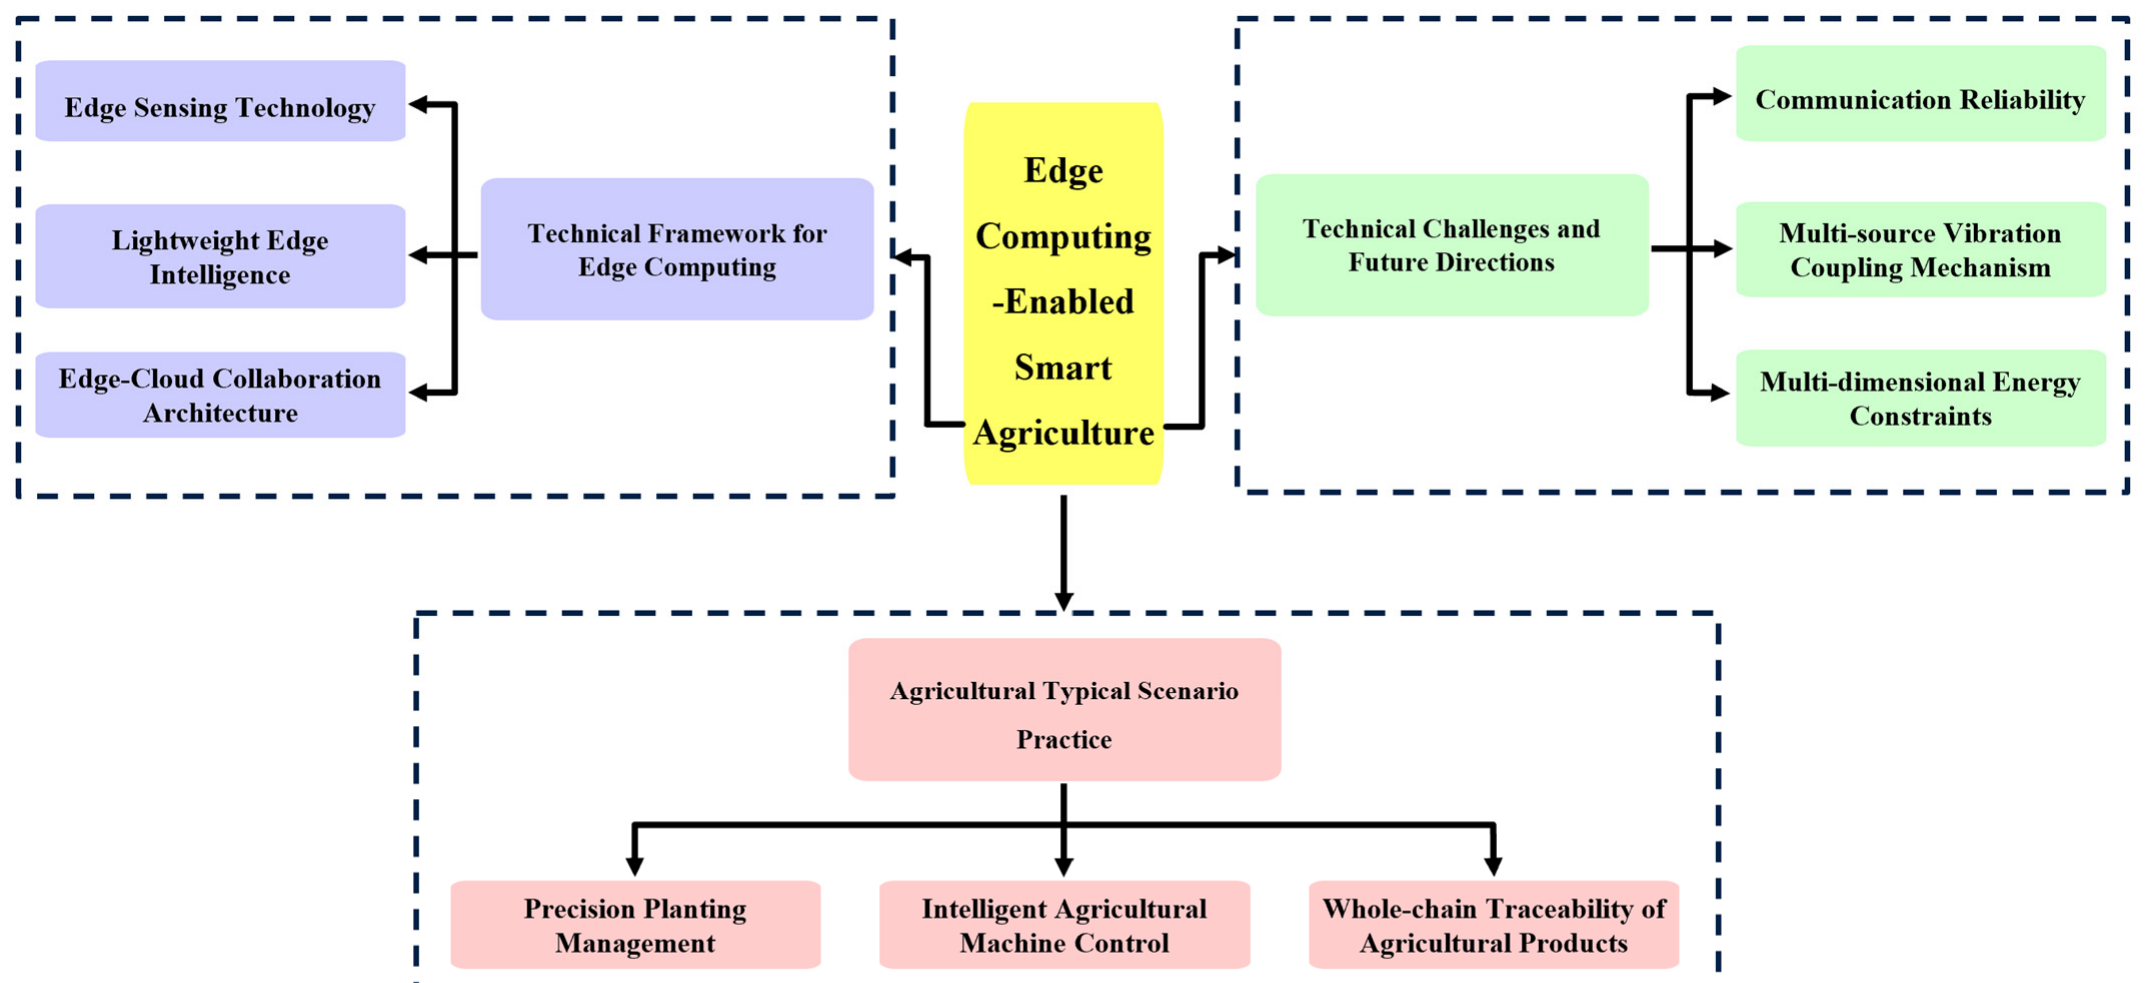
\includegraphics[width=0.95\textwidth]{figures/extracted/gong2025-edge-computing-framework.png}
  \caption{Edge computing framework for smart agriculture, reproduced
           under CC~BY~4.0 from~\cite{gong2025edge}.}
  \label{fig:edge-computing-framework}
\end{figure}

\ubsoft{Identity, Privacy and Access Control in Adjacent Domains}
\label{subsec:lit_privacy_extended}

The most developed treatment of identity and privacy over a permissioned ledger
comes from electronic health records, where the regulatory pressure is
greatest. \textcite{tang2019efficientauthentication} proposes an
authentication scheme binding records to enrolled principals;
\textcite{rajput2019eacmsemergency} adds emergency access control with
after-the-fact auditability; \textcite{yousif2026enablingprivacy} and
\textcite{hurdson2026enhancingelectronic} address external sharing without
disclosing the underlying record. \textcite{kormiltsyn2023privacyconflict}
treats the conflict that arises when personal and institutional records are
integrated, which is structurally the same problem as a farmer's data entering
a consortium ledger.

The agricultural instances are thinner but converge on the same requirement.
\textcite{ali2023farmDataTampering} addresses tampering in farm \gls{iot} data,
and \textcite{safeer2024tomato} reports a production deployment in the Italian
tomato chain. \textcite{aouedi2024surveyintelligent} and
\textcite{sahu2024exploringsecurity} survey the \gls{iot} threat surface and
agree that constrained endpoints remain the weakest link, which is the
observation Section~\ref{sec:problem} builds on.

Two limits recur across this literature. Authentication is enforced where
compute is available, that is at the gateway or the server, not at the sensing
node; and confidentiality is obtained by withholding data from the ledger,
which reintroduces a trusted party. Neither limit is addressed by a mechanism
that operates on the reading in flight.

\section{Research in Cognate Areas Relevant to the Topic}
\label{sec:lit_cognate}

Three adjacent bodies of work inform our work without belonging to any
of the themes surveyed above.

\textbf{General edge computing and \gls{iot} security}, beyond agriculture,
establishes both the promise and the residual risk of pushing computation
to the network edge. Edge processing improves response latency and keeps
sensitive data local~\cite{sharma2020edge, liu2019edge, wang2021edge}, and
this holds across smart-city and vehicular deployments as much as
agricultural ones, a distributed vehicular network architecture built on
Merkle-tree-verified blocks being one such
example~\cite{sharma2018merkle}. The security side of the same literature
catalogues \gls{iot}-specific attack surfaces, firmware injection,
authentication bypass and physical tampering among
them~\cite{hassan2019iotSecurity, dorri2017blockchain, kalaimathi2025injection, akande2018iotChallenges, knight2025iotResilience, bashir2023IoTWear}, and a smaller literature addresses the specific
hardware we deploy, cache and memory-region behaviour on the
ESP32 family, relevant to firmware-level integrity rather than network
protocol design~\cite{kumari2025rom, csdn_esp32s3_cache, esp_hal_cache}.

\textbf{Distributed and parallel computing beyond blockchain} supplies the
scaling vocabulary used in Section~\ref{subsec:lit_consensus} and in
Chapter Four: Amdahl's law bounds the speedup obtainable from
parallelising a fixed-size workload by the fraction that remains
sequential, a ceiling our strong-scaling analysis of gateway
count against transaction throughput invokes
directly~\cite{amdahl1967validity}. Ongoing revocation-latency work in
vehicular and other resource-constrained permissioned-blockchain settings
similarly treats edge computing as the deployment target rather than the
enterprise data centre~\cite{lu2022revocation}, reinforcing the pattern
Section~\ref{subsec:lit_consensus} identifies: constrained-hardware
evaluation is the literature's exception rather than its default.

\textbf{Applied hydrology and arid-region agronomy} ground our
water-efficiency claims outside the networking and ledger literature
proper. Global freshwater withdrawal projections identify irrigation as
the dominant consumptive use and the primary lever for closing the gap
between supply and demand under
population growth~\cite{fao2050, un_water2023}, and Mediterranean and North
African basin studies, including region-specific work on
Tunisia~\cite{tunisia_water_report, adeloye2021tunisiaAgro, benali2024tunisiaWater}, quantify the scale of the
shortfall our field site sits inside. Crop-specific water-stress
and quality studies for tomato and pepper cultivation, the two crops
monitored in our deployment, supply the agronomic baselines
against which Chapter Four's yield and water-use results are
compared~\cite{mdpi_tunisia_tomato, jaeid_pepper, fao_tomato_guide, safeer2024tomato, wang2025pepper, tia2020waterstress, pepper2021moisturecontrol, capsicumspacing2017study, precision2020yield, pepperquality2019irrigation}.

\section{Critique of Current Literature and Summary of Known Results}
\label{sec:lit_critique}

Read across the threads surveyed above, the literature is strong on
isolated mechanisms and weak on their combination and their field
validation. Table~\ref{tab:lit-gap-summary} states this critique per
thread in the same form our own contribution
(Section~\ref{sec:lit_contribution}) will answer it.

\begin{table}[htbp]
\centering
\caption{Critique of current literature by thread, and what remains
         unestablished}
\label{tab:lit-gap-summary}
\footnotesize
\begin{tabularx}{\textwidth}{@{}p{0.20\textwidth}X X@{}}
\toprule
\textbf{Thread} & \textbf{What the literature establishes} & \textbf{What remains unestablished} \\
\midrule
Precision agriculture \& \gls{iot} sensing (\S\ref{subsec:lit_precision_ag})
  & Sensor-driven scheduling reduces water use; decision-support benefit is
    replicated across regions
  & Data-integrity assumptions behind those results are rarely stated or
    measured; field sensing error budgets are under-reported \\
\midrule
\gls{lpwan} transmission \& energy (\S\ref{subsec:lit_lpwan})
  & Compression reduces payload; residue decomposition reduces storage and
    per-node energy in isolation
  & No prior system uses residue decomposition for concurrent multi-channel
    \emph{reception}, the mechanism that governs gateway capacity \\
\midrule
\gls{rns} / \gls{crt} in communications (\S\ref{subsec:lit_crt})
  & Reconstruction is exact and $O(k)$; subset recovery tolerates missing
    residues; parallel decomposition accelerates cryptographic verification
  & The processor-cycle application and the radio-channel application have
    not been connected; confidentiality implications of residue disclosure
    are unexploited \\
\midrule
Blockchain / \gls{dlt} in agriculture (\S\ref{subsec:lit_blockchain_ag})
  & Hash-chained, replicated ledgers give tamper evidence for agricultural
    and supply-chain records
  & Authentication almost universally terminates at the gateway or
    enterprise boundary, not the sensing node \\
\midrule
Edge-resident consensus (\S\ref{subsec:lit_consensus})
  & \gls{cft}/\gls{bft} trade-off is well characterised in message
    complexity; \gls{cap} constrains any partitioned deployment
  & Constrained \gls{arm64} gateway-class evaluation, especially under
    sustained field load rather than benchmark load, is the exception \\
\midrule
Identity, access control \& privacy (\S\ref{subsec:lit_privacy})
  & \gls{rbac}/\gls{msp} identity binding and role hierarchies are
    formalised and enforceable in chaincode
  & Node-level (not gateway-level) identity binding is largely absent;
    transmission-layer confidentiality is not treated as a design resource \\
\bottomrule
\end{tabularx}
\end{table}

Three cross-cutting patterns follow from the table. First, every thread
that reports a resource saving, transmission, storage, or processor
cycles, reports it in isolation, with no accounting of what that saving
could purchase elsewhere in the same pipeline; Section~\ref{sec:rationale}
of Chapter One turns this observation into our central rationale.
Second, authentication and consensus evaluation both stop at the gateway,
leaving the sensing node, the point at which falsification is cheapest,
outside the trust boundary the literature actually measures. Third,
laboratory and simulated evaluation dominates every thread; sustained
field deployment, of the kind Chapter Three's methodology and Chapter
Four's results describe, is reported by a minority of the studies
reviewed here, and by none that combine transmission efficiency, edge
consensus and access control in a single system.

\section{Research Frontiers}
\label{sec:lit_frontiers}

Four questions are live in the literature discussed above and unresolved in it.

\textbf{Whether decomposition can serve efficiency and confidentiality at
once.} Residue representations are used for throughput in the ledger
literature~\cite{horvath2025assistedsharding, patel2023blockchainlayer} and,
separately, for concealment in the image-security
literature~\cite{yavuz2025reversibledata}. No work discussed here establishes
the two properties for a single decomposition under one threat model.

\textbf{How far identity can be pushed toward the sensor.} Every scheme
surveyed in Section~\ref{subsec:lit_privacy_extended} terminates authentication
at a device with meaningful compute. Whether a node with a few kilobytes of
free memory can carry a credential strong enough to bind an individual reading,
and at what airtime cost, is open.

\textbf{What permissioned consensus actually costs in the
field.} Benchmarks now exist for constrained
hardware~\cite{zulkarnain2025performancebenchmarking, pebriyanti2025evaluationscalability}, but they are laboratory measurements.
Behaviour under mesh partition, thermal derating and seasonal power variation
is reported nowhere in this body of work.

\textbf{Where the binding constraint sits as deployments grow.}
Equations~\ref{eq:lora_airtime} and~\ref{eq:mdOne} are sensitive to
different quantities, so node-count and packet-capacity limits bind under
different conditions. No validated model in prior work distinguishes
them for multi-channel residue traffic.

\section{The Contribution This Study Will Make to the Literature}
\label{sec:lit_contribution}

Against the gaps summarised in Table~\ref{tab:lit-gap-summary}, we
contribute the following.

\begin{enumerate}
  \item We connect the processor-cycle application of \gls{crt} parallel
        decomposition that the residue-arithmetic literature establishes
        (Section~\ref{subsec:lit_crt}) to a radio-channel application,
        showing that Equation~\ref{eq:crt_reconstruction} pays for a
        different resource, airtime rather than \gls{cpu} cycles, when its
        parallel targets are a concentrator's demodulation paths rather
        than a processor's cores.
  \item We extend gateway-terminated identity binding to the sensing
        node, using the hierarchical \gls{rbac} formalisation of
        Equations~\ref{eq:hrbac_eff} and~\ref{eq:hrbac_grant}
        (Appendix~\ref{app:hrbac_matrix}) together with per-node
        credentials, so that a ledger record attests to the node that
        produced a reading rather than only to the gateway that submitted
        it.
  \item We report \gls{cft} consensus performance measured on \gls{arm64}
        gateway hardware under sustained field load rather than benchmark
        or simulated load, addressing the field-validation gap
        Table~\ref{tab:lit-consensus} identifies across the consensus
        literature.
  \item We state, and Chapter Four tests as hypothesis H5, the condition
        under which residue decomposition can serve as a confidentiality
        substrate rather than merely a transmission optimisation: that
        disclosure from an intercepted residue is bounded by the ratio
        between the plaintext domain and the missing moduli's product, a
        condition the subset-recovery results
        of~\cite{goldreich1999china, shoup2009computational} make precise
        but do not by themselves establish for any deployed system,
        connecting the transmission and privacy threads that
        Section~\ref{subsec:lit_privacy} shows have developed
        separately.
  \item We report the combined system, transmission, ledger and access
        control, characterised together on one deployment, rather than
        each mechanism validated in isolation, which
        Section~\ref{sec:lit_critique} identifies as the pattern prior
        work does not yet show.
\end{enumerate}

\section{Partial Conclusion}
\label{sec:lit_partial_conclusion}

The sensing literature has solved measurement and left trust untouched: the
reading is believed because it was reported, and no mechanism attests that the
value stored is the value measured~\cite{soussi2024smartsensors, aydin2021comprehensive}. The transmission literature has correctly identified
airtime as the binding constraint and attacks it by shortening payloads, which
reduces total volume but not the per-packet occupancy that
the duty-cycle and airtime relations of Equations~\ref{eq:duty_cycle}
and~\ref{eq:lora_airtime} are actually sensitive to~\cite{marcelloni2009energy, chen2025compression}. Residue arithmetic
supplies a decomposition whose parallelism has been exploited in silicon and,
recently, in ledger throughput, but never on the
air~\cite{parhami2010computer, luo2023researchapplication, maiwada2025blockchainscalability}. The ledger literature supplies tamper
evidence and an identity layer, characterised on hardware that agricultural
deployments do not have~\cite{tar2023fabric, zulkarnain2025performancebenchmarking}. The privacy literature obtains
confidentiality by withholding, which forfeits the verifiability that motivated
the ledger in the first place~\cite{kormiltsyn2023privacyconflict, yousif2026enablingprivacy}.

Taken together these five leave one composite question, which we address in
the chapters that follow: whether a decomposition adopted to reduce per-packet
occupancy can simultaneously carry node-level identity and bound disclosure,
and whether the resulting system holds up on the hardware and under the
conditions that field deployment actually imposes.
